\chapter{Introduction}
\label{ch:intro}

\noindent \emph{Orthogonal range searching} is one of the most fundamental and well-studied problems in computational geometry. Even with extensive research over three decades a lot of questions remain. In this thesis we will focus on $2D$ orthogonal range searching: Given $n$ points from $\mathbb{R}^2$ we want to insert them into a data structure which will be able to efficiently report which points lie within a given axis-aligned query rectangle $\mathbb{Q} \subseteq \mathbb{R}^2$.

\begin{figure}[h]
    \centering
    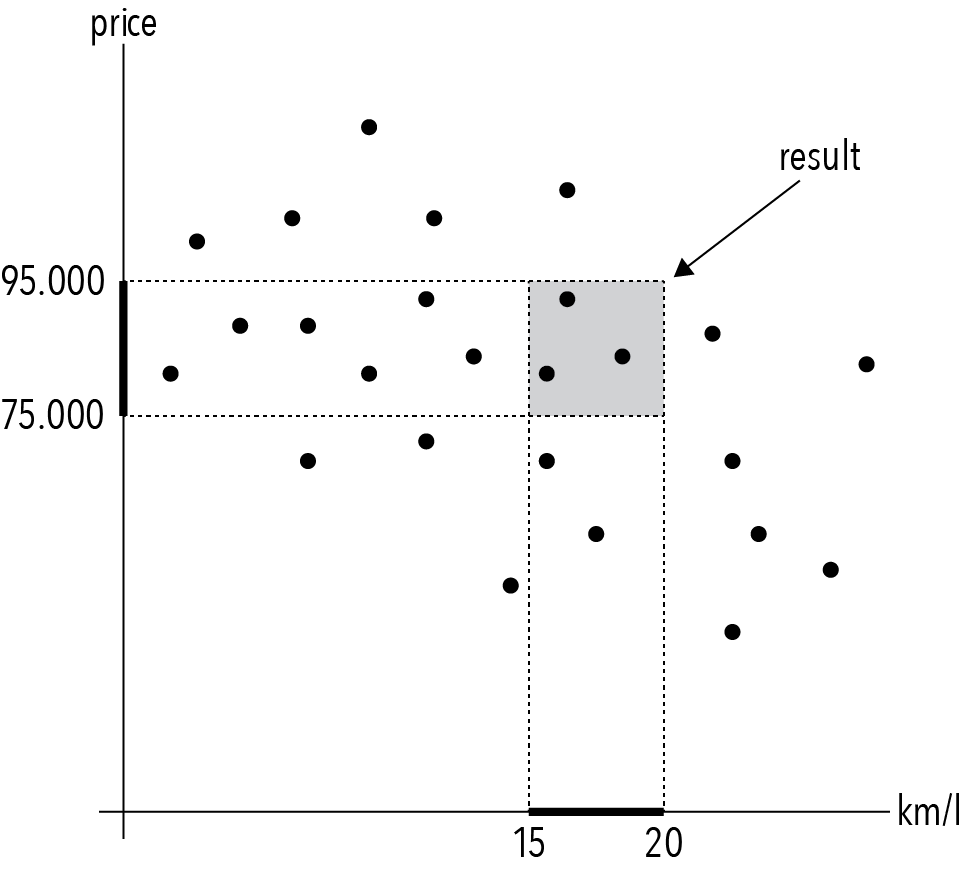
\includegraphics[width = 0.75\textwidth]{pictures/introduction.png}
    \caption{Example of an orthogonal range query}\label{fig:example}
\end{figure}

\noindent To motivate the problem, consider a database of vehicles for sale. Each vehicle has measurable attributes like price, the year the model was released, engine size, amount of doors, gasoline consumption in kilometers per liter, size  and maximum speed. Perhabs a buyer is interested in finding cars which cost between $75,000$ and $95,000$ and can drive between $15$ and $20$ kilometers per liter of gasolin. We can see such a search on figure~\ref{fig:example}, where each point within the gray area represents a car which fits the criteria, i.e. a search on two parameters is equivalent to finding all points within a $2$-dimensional orthogonal range query. When performing a seach, two attributes are picked and a range for both attributes can be set, giving a $2$-dimensional search query. A point in the graph reprensents the ID of the car with which the car can be looked up in the database to find the other attributes of the car. We can think of each car as a point with one coordinate per attribute. Given the ranges of two attributes we want to find those of the cars in the database which lie within the search query. In the example on figure~\ref{fig:example} the search range is the $2$d rectangle $[15;20] \times [75,000;95,000]$ returning three cars as the result. \\

The objective of this thesis is to study a variety of \emph{orthogonal range searching} data structures. The main focus will be to introduce the \emph{Simple Range Search} data structure. It is a simplification of an orthogonal range searching data structure by \citet{chanetal}, which will be referred to as the \emph{Original Range Search} data structure. We are going to describe the kd-tree which will be the reference data structure in our analysis of the Simple Range Search data structure. We are going to describe the range tree which shares some of properties of the Simple Range Search and Original Range Search data structures.

We show that a range query to the Simple Range Search data structure has a faster worst-case running time than a range query to the kd-tree. We also show that the Simple Range Search data structure is able to compete with the kd-tree, and even strongly outperform the kd-tree in cases where the shape of the query is a long thin slice through the attribute area. \todo{Andet ord} \\ 


The model of computation used in this thesis is the $w$-bit word-RAM model by \citet{fredman}. In the word-RAM model of computation, the memory is divided into words of $w$ bits. Given a set $P$ of $n$ points with coordinates from a universe $U$, a word will have enough bits to store the integer address of any index into $P$ and enough bits to store any element from $U$. Thus, $w = \Omega(\lg n)$ and $w = \Omega(\lg U)$. Under the word-RAM model all standard word operations take constant time. This includes standard word operation from modern programming languages such as integer addition, subtraction, multiplication, division, shifts and the bit-wise operators AND, OR and XOR. Reading a single word from memory or writing a single word to memory also takes constant time. The number of bits in a word is found by the largest element which has to fit into a word. This means that it is often possible to divide the word into smaller logical blocks which can fit more than one integer. \\ 


\noindent \textbf{Outline.} Has yet to be written. \\

\noindent \textbf{Notation.} The set of integers $\{i, i+1, \dots, j-1, j\}$ is denoted by $[i,j]$. When no base is explicitely given logarithm will have base $2$. $\epsilon$ is an arbitrary small constant greater than $0$. Given an array $A$, $A[i]$ denotes the entry with index $i$ in $A$ and $A[i,j]$ denotes the subarray containing the entries from $i$ to $j$ in $A$, including both $A[i]$ and $A[j]$. $A[1..n]$ denotes an array $A$ of size $n$ with entries $1$ to $n$. Throughout the thesis the successor of $x$ in a set will be meant as the smallest number which is greater or equal to $x$ in that set - symmetrically, the same applies for predecessor of $x$ which is the biggest number less or equal to $x$. The work will be done under the assumption that no two points will  have the same x-coordinate and no two points will have the same y-coordinate. This is a unrealistic assumption in practice, but it can easily be remedied by having the points lie in a \emph{composite-number space} since we only need a total ordering of our points.



